\documentclass{article}
\usepackage[utf8]{inputenc}
\usepackage{titling}
\usepackage{graphicx}
\usepackage{xcolor}
\usepackage[colorlinks=true,linkcolor=darkgray, urlcolor =gray]{hyperref}
\usepackage[spanish]{babel}
\DeclareUnicodeCharacter{301}{~}
\usepackage{url}


\title{Práctica 1. Introducción de redes bayesianas en el programa GeNIe}
\author{Cristina Díaz García}
\date{Marzo 2019}

\renewcommand\maketitlehooka{\null\mbox{}\vfill}
\renewcommand\maketitlehookd{\vfill\null}


\begin{document}

\addcontentsline{toc}{section}{Índice general}

\begin{titlingpage}
\maketitle
\end{titlingpage}

\newpage

\tableofcontents

\newpage

\section{Enunciado}

\textbf{\underline{Tarea:}} Para los siguientes enunciados, modela el problema como una red bayesiana e introdúcelo en GeNIe.

\textbf{\underline{Entrega:}} Documento pdf, que contenga capturas de la imagen de los modelos y de las tablas de probabilidad (sólo de los nodos con padres) de cada una de las cuatro redes de los enunciados.

\section{Ejercicio 1}

Considera la siguiente situación: Los padres de Luisito, que acaba de cumplir un año, deciden
llevarlo al pediatra porque vomita con cierta frecuencia. Con el pediatra sostienen la siguiente conversación:

\textit{Pediatra -. Denme toda la información que consideren que puede ser relevante.\\}
\textit{Mamá-. El otro día Luisito estaba resfriado. Vomitó el biberón de la noche, creo que por culpa de los mocos, ya que había muchos en el vómito. Otras veces parece que vomita por una pequeña indigestión.\\}
\textit{Papá-. Además, creo que debe saber que mi hermano es celíaco (Aclaración: la celiaquía es una intolerancia al gluten, que poco a poco hace que se destruya el vello intestinal. Los vómitos son uno de sus síntomas más relevantes. Se cree que tiene cierta componente hereditaria).\\}
\textit{Pediatra-. ¿Y la dieta de Luisito incluye gluten?\\}
\textit{Ambos-. Sí, desde hace unos meses.}

\subsection{Solución proporcionada}

\textbf{Modelo general}

\begin{center}
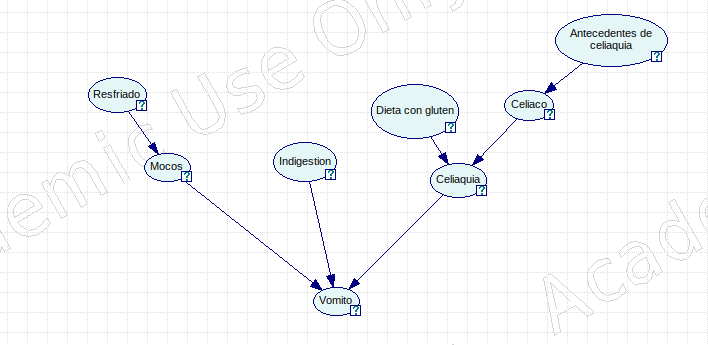
\includegraphics[scale=0.5]{Modelo1.png}
\end{center}

\newpage

\textbf{Tabla de propabilidad de \textit{Celiaco}}

\begin{center}
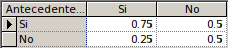
\includegraphics[scale=0.5]{Celiaco.png}
\end{center}

\textbf{Tabla de propabilidad de \textit{Celiaquía}}

\begin{center}
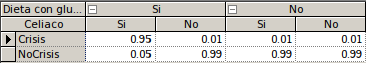
\includegraphics[scale=0.5]{Celiaquia.png}
\end{center}

\textbf{Tabla de propabilidad de \textit{Mocos}}

\begin{center}
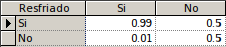
\includegraphics[scale=0.5]{Mocos.png}
\end{center}


\textbf{Tabla de propabilidad de \textit{Vomito}}

\begin{center}
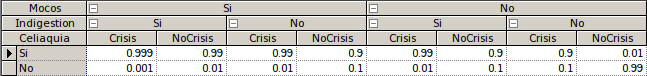
\includegraphics[scale=0.5]{Vomito.png}
\end{center}

\section{Ejercicio 2}

En el planeta Zyx se pueden encontrar varias clases de animales, llamemos a estas clases Wurros,
Hobexas y Wackas. Todos tienen un tamaño muy pequeño, y sus pieles son o bien escamosas obien están cubiertas de suave pelo. Además, una observación atenta ha permitido deducir lo
siguiente:\\
• Todos los Wurros tienen 5 ó 6 patas. Su color es rojizo, y tienen la piel peluda y suave.\\
• El número de patas de las Hobexas es un entero que varía uniformemente entre 4 y 6,
ambos inclusive. Su piel es escamosa.\\
• En cuanto a las Wackas, tienen 4 ó 5 patas, y ofrecen a la vista una tonalidad casi siempre
azul, pero a veces (20\% de los casos) rojiza.\\
• Los animales que tienen un número impar de patas cojean siempre. Los animales que
tienen un número par de patas cojean sólo cuando tienen alguna anomalía (malformación
congénita, heridas, etc.), lo cual ocurre en el 10\% de los casos para los animales de 4 patas, y en el 20\% para los de seis.\\
Plantea el problema de la clasificación de animales de Zyx mediante una red bayesiana
Nota: este problema admite dos modelos correctos, uno que incluye el nodo anomalía y otro que modela las anomalías a través de las probabilidades condicionadas. Se pide introducir ambos modelos.

\subsection{Solución proporcionada}

\textbf{Modelo con Anomalía}

\begin{center}
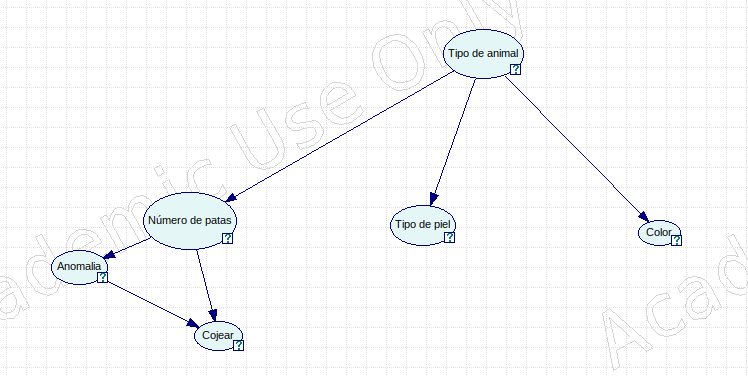
\includegraphics[scale=0.5]{Modelo2.png}
\end{center}

\textbf{Tabla de propabilidad de \textit{Color}}

\begin{center}
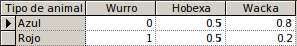
\includegraphics[scale=0.5]{Color.png}
\end{center}

\textbf{Tabla de propabilidad de \textit{Tipo de piel}}

\begin{center}
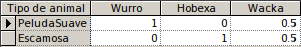
\includegraphics[scale=0.5]{piel.png}
\end{center}

\textbf{Tabla de propabilidad de \textit{Número de patas}}

\begin{center}
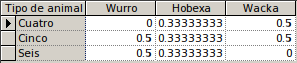
\includegraphics[scale=0.5]{Patas.png}
\end{center}

\textbf{Tabla de propabilidad de \textit{Anomalia}}

\begin{center}
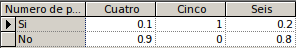
\includegraphics[scale=0.5]{Anomalia.png}
\end{center}

\newpage

\textbf{Modelo sin Anomalía}

\begin{center}
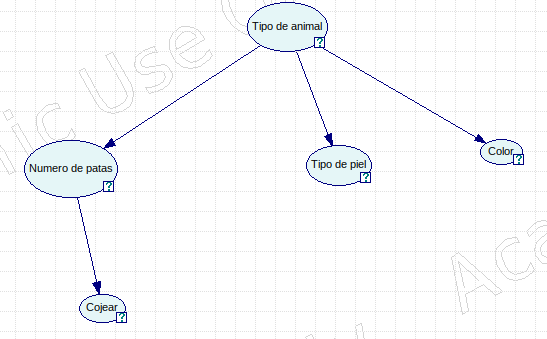
\includegraphics[scale=0.5]{Modelo2b.png}
\end{center}

\textbf{Tabla de propabilidad de \textit{Color}}

\begin{center}
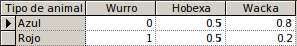
\includegraphics[scale=0.5]{Color.png}
\end{center}

\textbf{Tabla de propabilidad de \textit{Tipo de piel}}

\begin{center}
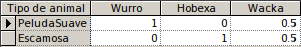
\includegraphics[scale=0.5]{piel.png}
\end{center}

\textbf{Tabla de propabilidad de \textit{Número de patas}}

\begin{center}
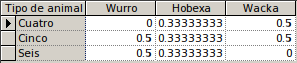
\includegraphics[scale=0.5]{Patas.png}
\end{center}

\section{Ejercicio 3}

Una tarde, Luis va a visitar a su compañero de oficina Antonio, y de repente comienza a
estornudar. Luis piensa que se ha resfriado. Pero de repente observa que los muebles de Antonio están arañados, de forma que se le ocurre que quizás su amigo tenga un gato y sus estornudos se deban a una crisis producida por una rinitis alérgica.

\newpage

\subsection{Solución proporcionada}

\textbf{Modelo general}

\begin{center}
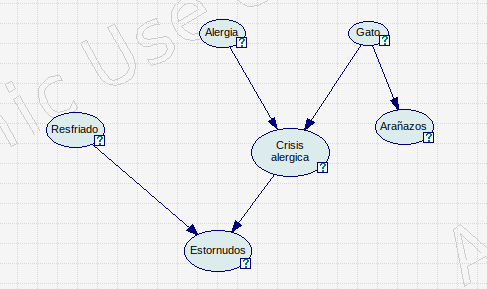
\includegraphics[scale=0.5]{Modelo3.png}
\end{center}

\textbf{Tabla de propabilidad de \textit{Arañazos}}

\begin{center}
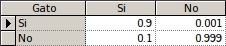
\includegraphics[scale=0.5]{Gato.png}
\end{center}

\textbf{Tabla de propabilidad de \textit{Crisis alérgica}}

\begin{center}
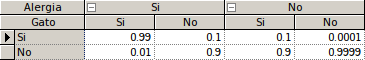
\includegraphics[scale=0.5]{Crisis.png}
\end{center}

\textbf{Tabla de propabilidad de \textit{Estornudos}}

\begin{center}
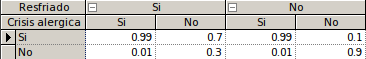
\includegraphics[scale=0.5]{Estornudos.png}
\end{center}

\section{Ejercicio 4}

El problema de Monty Hall. A un concursante del concurso televisivo Let ́s Make a Deal se le pide que elija una puerta entre tres (todas cerradas), y su premio consiste en llevarse lo que se encuentra detrás de la puerta elegida. Se sabe que una de ellas oculta un coche, y las otras dos tienen una cabra. Una vez que el concursante ha elegido una puerta y le comunica al público y al presentador su elección, el presentador (que conoce en que puerta está el premio) abre una de las otras puertas y muestra una cabra. En este momento se le da la opción al concursante de quedarse con la puerta que eligió inicialmente o bien cambiar de puerta. ¿Debe el concursante cambiar de puerta, o mantener su elección?

\subsection{Solución proporcionada}

\textbf{Modelo general}

\begin{center}
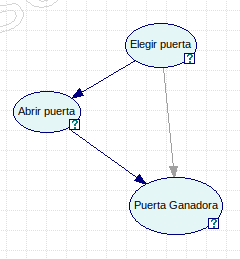
\includegraphics[scale=0.5]{Modelo4.png}
\end{center}

\textbf{Tabla de propabilidad de \textit{Abrir Puerta}}

\begin{center}
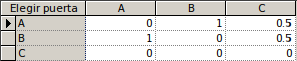
\includegraphics[scale=0.5]{Abrir.png}
\end{center}

\textbf{Tabla de propabilidad de \textit{Puerta Ganadora}}

\begin{center}
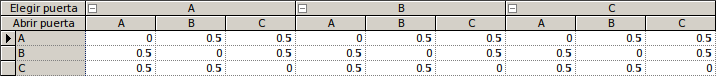
\includegraphics[scale=0.5]{Ganadora.png}
\end{center}

\section{Ejercicio 5}

Juan y Luisa llegan un día a casa y observan que el coche no está en el garaje, con lo cual piensan que se lo han robado. Cuando Juan está a punto de llamar a la policía, Luisa le dice que no llame, ya que es probable que haya sido María (su hija adolescente) la que haya cogido el coche sin permiso: Juan le pregunta qué le hace pensar eso, y Luisa responde que, además de que el coche de María está en el taller, esa misma mañana María recibió una misteriosa llamada telefónica, lo cual indica que quizás tuviera una cita importante para la que necesitara el coche.

\newpage

\subsection{Solución proporcionada}

\textbf{Modelo general}

\begin{center}
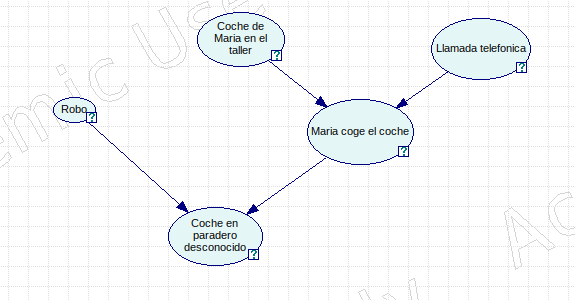
\includegraphics[scale=0.5]{Modelo5.png}
\end{center}

\textbf{Tabla de propabilidad de \textit{Maria coge el coche}}

\begin{center}
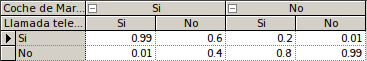
\includegraphics[scale=0.5]{MariaCoche.png}
\end{center}

\textbf{Tabla de propabilidad de \textit{Coche en paradero desconocido}}

\begin{center}
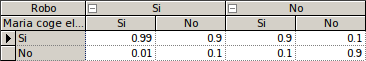
\includegraphics[scale=0.5]{CocheDesaparecido.png}
\end{center}

\section{Ejercicio 6}

Juan está en la parada del autobús de la línea 20, y el autobús se está retrasando. Juan piensa que puede que haya retenciones de tráfico, pero también puede ser que el autobús haya sufrido una avería o que hayan suspendido el servicio de la línea por las obras del metro. El servicio de una línea se suspende cuando hay obras que la afectan y hay otras líneas en servicio que pueden utilizar los usuarios para sus desplazamientos.

\newpage

\subsection{Solución proporcionada}

\textbf{Modelo general}

\begin{center}
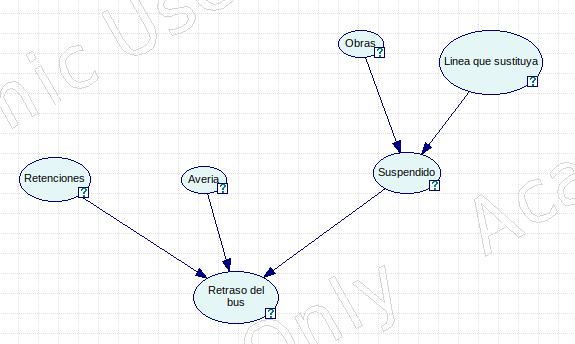
\includegraphics[scale=0.5]{Modelo6.png}
\end{center}

\textbf{Tabla de propabilidad de \textit{Suspendido}}

\begin{center}
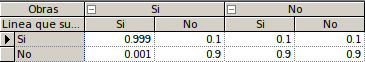
\includegraphics[scale=0.5]{Suspendido.png}
\end{center}

\textbf{Tabla de propabilidad de \textit{Retraso del bus}}

\begin{center}
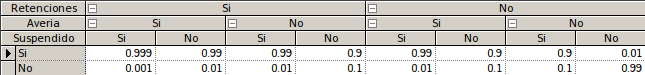
\includegraphics[scale=0.5]{Retraso.png}
\end{center}

\section{Ejercicio 7}

La policía está intentando establecer un modelo que permita razonar sobre los accidentes de
tráfico causados por una pérdida de control del vehículo del conductor. Esta pérdida de control suele venir provocada por un error humano, una carretera resbaladiza, un fallo mecánico o un exceso de velocidad. El error humano suele deberse a una distracción del conductor y una capacidad de reacción mermada por alguna circunstancia (consumo de sustancias o cansancio). La carretera puede estar resbaladiza por vertido de sustancias o por las condiciones atmosféricas.

\newpage

\subsection{Solución proporcionada}

\textbf{Modelo general}

\begin{center}
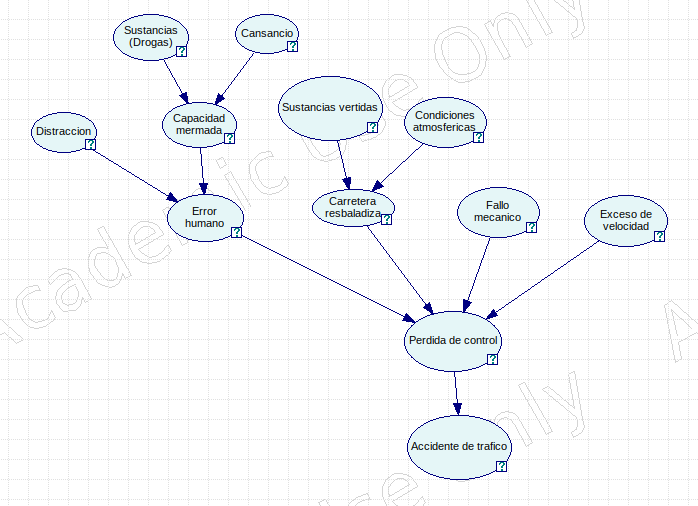
\includegraphics[scale=0.5]{Modelo7.png}
\end{center}

\textbf{Tabla de propabilidad de \textit{Capacidad mermada}}

\begin{center}
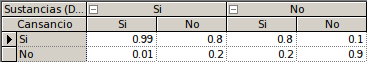
\includegraphics[scale=0.5]{Capacidad.png}
\end{center}

\textbf{Tabla de propabilidad de \textit{Error humano}}

\begin{center}
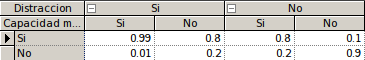
\includegraphics[scale=0.5]{Error.png}
\end{center}

\textbf{Tabla de propabilidad de \textit{Carretera resbaladiza}}

\begin{center}
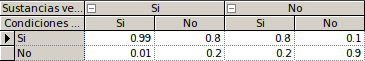
\includegraphics[scale=0.5]{Carretera.png}
\end{center}

\textbf{Tabla de propabilidad de \textit{Pérdida de control}}

\begin{flushleft}
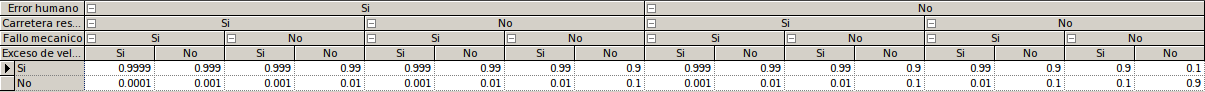
\includegraphics[scale=0.35]{Control.png}
\end{flushleft}

\textbf{Tabla de propabilidad de \textit{Accidente de tráfico}}

\begin{center}
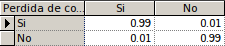
\includegraphics[scale=0.5]{Accidente.png}
\end{center}

\begin{thebibliography}{9}
\bibitem{Bayes} Información oficial de GeNIe, \url{https://www.bayesfusion.com}.
\end{thebibliography}

\end{document}